\documentclass[12pt,a4paper]{report}

% ---------------------------------------------------------
% PAQUETES
% ---------------------------------------------------------
\usepackage[utf8]{inputenc}
\usepackage[T1]{fontenc}
\usepackage[spanish]{babel}
\usepackage{geometry}
\usepackage{setspace}
\usepackage{graphicx}
\usepackage{hyperref}
\usepackage{booktabs}
\usepackage{float}
\usepackage{array}
\usepackage{tabularx}
\usepackage{listings}
\usepackage{xcolor}

\geometry{margin=2.5cm}
\setstretch{1.5}

\hypersetup{
    colorlinks=true,
    linkcolor=blue,
    urlcolor=blue,
    citecolor=blue
}

\lstset{
    basicstyle=\ttfamily\footnotesize,
    breaklines=true,
    frame=single,
    backgroundcolor=\color{gray!10},
    showstringspaces=false
}

\renewcommand{\thesection}{\arabic{section}}
\renewcommand{\thesubsection}{\thesection.\arabic{subsection}}

\begin{document}

% ---------------------------------------------------------
% PORTADA
% ---------------------------------------------------------
\begin{titlepage}
    \centering

    \begin{minipage}{0.45\textwidth}
        \centering
        \includegraphics[width=0.8\textwidth]{logo_utb.png}
    \end{minipage}
    \hfill
    \begin{minipage}{0.45\textwidth}
        \centering
        \includegraphics[width=0.8\textwidth]{logo_escuela.png}
    \end{minipage}

    \vspace{1.5cm}

    {\Large Universidad Tecnológica de Bolívar\\[0.5cm]
    Escuela de Transformación Digital}\\[2cm]

    {\bfseries\LARGE Proyecto 04 -- Plataforma de Almacenamiento\\de Objetos con CDN Global\\y Ciclo de Vida en AWS\\[0.5cm]}
    {\large (Infraestructura como Código -- Terraform + AWS)}\\[2cm]

    {\large Estudiantes:\\
    \textbf{Manuel Esteban Severiche Puello\\
    Angel Jhoan Acero Martinez\\
    Jerson David Diaz Alvarez\\
    Julio De Jesus Denubila Vergara\\
    Diego Jose Marin Sara}}\\[0.8cm]

    {\large Curso:\\
    \textbf{Infraestructura}}\\[0.8cm]

    {\large Docente:\\
    \textbf{Rafael Enrique Monterroza Barrios}}\\[0.8cm]

    \vfill
\end{titlepage}

% ---------------------------------------------------------
% ÍNDICE
% ---------------------------------------------------------
\tableofcontents
\clearpage

% =========================================================
% 1. DESCRIPCIÓN DEL PROYECTO
% =========================================================
\section{Descripción del Proyecto}

Construcción de una plataforma de almacenamiento y distribución de contenido estático en Amazon Web Services, totalmente provisionada mediante Infraestructura como Código (Terraform) y desplegada continuamente a través de un pipeline de GitHub Actions con federación OIDC. La solución integra Amazon S3 (hosting y archivado), CloudFront (CDN global), Lambda@Edge (headers de seguridad) y políticas de ciclo de vida que migran los objetos entre clases de almacenamiento para optimizar costos.

El caso de uso es la distribución de contenido estático y archivos de usuario con baja latencia global, cifrado en reposo, HTTPS obligatorio y automatización completa del despliegue.

% =========================================================
% 2. ARQUITECTURA Y SERVICIOS AWS
% =========================================================
\section{Arquitectura y Servicios AWS}

\begin{table}[H]
    \centering
    \caption{Servicios AWS utilizados.}
    \begin{tabular}{ll}
        \toprule
        \textbf{Servicio} & \textbf{Rol en el proyecto} \\
        \midrule
        Amazon S3 (assets)       & Hosting de contenido estático con OAC \\
        Amazon S3 (uploads)      & Archivos de usuario con lifecycle a Glacier \\
        Amazon S3 (logs)         & Logs de acceso de CloudFront \\
        Amazon CloudFront        & Red de distribución de contenido (CDN) global \\
        AWS Lambda@Edge          & Inyección de headers de seguridad HTTP \\
        AWS Certificate Manager  & Certificados TLS (solo con dominio propio) \\
        AWS IAM + OIDC           & Federación GitHub Actions $\rightarrow$ AWS \\
        Amazon DynamoDB          & Lock del estado de Terraform \\
        Terraform                & Infraestructura como Código \\
        GitHub Actions           & Pipeline CI/CD \\
        \bottomrule
    \end{tabular}
\end{table}

\subsection{Diagrama de arquitectura}

\begin{verbatim}
Usuario  --->  CloudFront Distribution  --->  Lambda@Edge (viewer-response)
                      |                               |
                      |                               +--> HSTS / CSP / XFO ...
                      v
               S3 Bucket (assets) con OAC
                      |
                      +--> SSE-S3 / Versionado / Block Public Access

       Bucket uploads:  Standard -> IA (30d) -> Glacier (90d) -> Delete (180d)
       Bucket logs   :  retencion 90 dias, privado
\end{verbatim}

% =========================================================
% 3. PROCESO DE DESPLIEGUE
% =========================================================
\section{Proceso de Despliegue}

Se ejecutaron los siguientes pasos para llevar el proyecto de repositorio vacío a un CDN funcionando en producción:

\begin{enumerate}
    \item \textbf{Bootstrap de estado remoto} (\texttt{scripts/bootstrap.sh}): creación del bucket S3 para el \textit{state} de Terraform y de la tabla DynamoDB para \textit{state locking}.
    \item \textbf{Federación OIDC GitHub $\rightarrow$ AWS}: creación del \textit{OIDC provider} \texttt{token.actions.githubusercontent.com} y del rol IAM \texttt{github-actions-p04-deploy} con \textit{trust policy} restringida al repositorio \texttt{Manuuell/p04-s3-cloudfront-cdn} mediante \texttt{StringLike} sobre el claim \texttt{sub}.
    \item \textbf{Empaquetado de Lambda@Edge}: construcción local del ZIP de \texttt{lambda/security-headers} (Node.js 20, sin dependencias externas).
    \item \textbf{Provisionamiento con Terraform}: \texttt{terraform init}, \texttt{plan} y \texttt{apply} sobre los módulos \texttt{s3}, \texttt{cloudfront}, \texttt{lambda-edge} e \texttt{iam}. Se crearon 19 recursos sin errores.
    \item \textbf{Publicación del sitio}: \texttt{aws s3 sync web/ s3://<assets>} e invalidación de CloudFront (\texttt{/*}) desde el pipeline.
    \item \textbf{Verificación}: escaneo en \url{https://securityheaders.com}, medición de latencias con \texttt{curl} y consulta de métricas en CloudWatch.
\end{enumerate}

\subsection{Decisiones de arquitectura relevantes}

\begin{itemize}
    \item Se utilizó \textbf{OAC (Origin Access Control)} en lugar del deprecado OAI, siguiendo la recomendación actual de AWS.
    \item El dominio personalizado se convirtió en \textbf{opcional} mediante la variable \texttt{use\_custom\_domain}. En la configuración \texttt{dev} quedó en \texttt{false}, usando el dominio por defecto \texttt{*.cloudfront.net}.
    \item El pipeline evita \texttt{workflow\_run} con \texttt{download-artifact}, que es inestable; en su lugar, \texttt{publish.yml} se dispara en \texttt{push} a \texttt{main} con \texttt{paths} filter.
\end{itemize}

% =========================================================
% 4. VERIFICACIÓN DEL DESPLIEGUE
% =========================================================
\section{Verificación del Despliegue}

\subsection{Infraestructura aplicada con Terraform}

Se ejecutó \texttt{terraform apply} sobre el ambiente \texttt{dev} creando los tres buckets, la distribución CloudFront, la función Lambda@Edge, la OAC y los roles IAM correspondientes.

\begin{figure}[H]
    \centering
    \includegraphics[width=0.95\textwidth]{p04_terraform_apply.png}
    \caption{Salida de \texttt{terraform apply} con 19 recursos creados.}
\end{figure}

\subsection{CDN sirviendo contenido estático}

La distribución CloudFront quedó disponible en \texttt{https://d14x2vaw9f2mo1.cloudfront.net}, enrutando peticiones al bucket privado de assets a través de OAC.

\begin{figure}[H]
    \centering
    \includegraphics[width=0.95\textwidth]{p04_cloudfront_site.png}
    \caption{Sitio servido a través de CloudFront con HTTPS.}
\end{figure}

\subsection{Headers de seguridad -- Grade A+ en securityheaders.com}

La Lambda@Edge \texttt{security-headers} inyecta seis cabeceras en cada respuesta (\textit{viewer-response}), obteniendo la máxima calificación en \url{https://securityheaders.com}.

\begin{figure}[H]
    \centering
    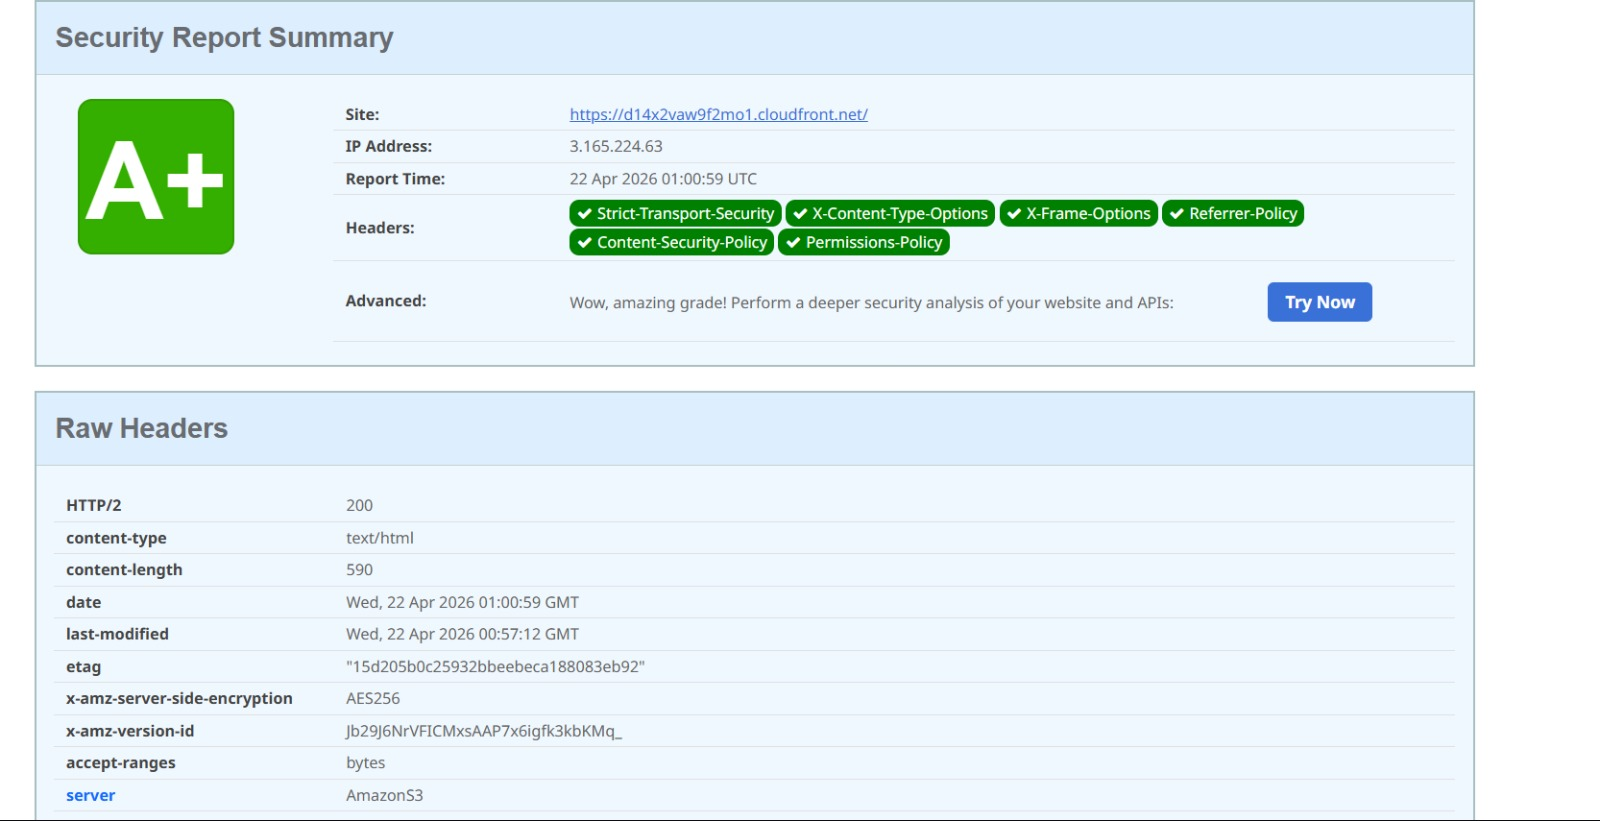
\includegraphics[width=0.95\textwidth]{securityheaders-aplus.jpg}
    \caption{Resultado A+ en securityheaders.com sobre \texttt{d14x2vaw9f2mo1.cloudfront.net}.}
\end{figure}

\begin{table}[H]
    \centering
    \caption{Headers de seguridad inyectados por la Lambda@Edge.}
    \begin{tabular}{p{4.5cm}p{8.5cm}}
        \toprule
        \textbf{Header} & \textbf{Valor} \\
        \midrule
        Strict-Transport-Security & \texttt{max-age=63072000; includeSubDomains; preload} \\
        X-Content-Type-Options    & \texttt{nosniff} \\
        X-Frame-Options           & \texttt{DENY} \\
        Referrer-Policy           & \texttt{strict-origin-when-cross-origin} \\
        Content-Security-Policy   & \texttt{default-src 'self'; ...} \\
        Permissions-Policy        & \texttt{camera=(), microphone=(), geolocation=()} \\
        \bottomrule
    \end{tabular}
\end{table}

\subsection{Pipeline de CI/CD en verde}

El workflow \texttt{publish.yml} ejecuta tests de Lambda, asume el rol vía OIDC, sincroniza \texttt{web/} con el bucket de assets e invalida el caché de CloudFront. Duración típica: 23 segundos.

\begin{figure}[H]
    \centering
    \includegraphics[width=0.95\textwidth]{p04_pipeline_green.png}
    \caption{Pipeline de GitHub Actions ejecutándose exitosamente en \textit{push} a \texttt{main}.}
\end{figure}

% =========================================================
% 5. ANÁLISIS DE COSTOS -- STANDARD vs IA vs GLACIER
% =========================================================
\section{Análisis de Costos: Standard vs IA vs Glacier}

Uno de los entregables clave del proyecto es la optimización de costos a través del ciclo de vida de S3. La siguiente tabla compara las clases de almacenamiento utilizadas (tarifas en USD por GB-mes, región \texttt{us-east-1}, abril 2026).

\begin{table}[H]
    \centering
    \caption{Comparación de clases de almacenamiento S3 en \texttt{us-east-1}.}
    \begin{tabular}{p{3.8cm}p{2.2cm}p{2.2cm}p{4.5cm}}
        \toprule
        \textbf{Clase} & \textbf{USD/GB-mes} & \textbf{Min. storage} & \textbf{Caso de uso} \\
        \midrule
        S3 Standard                  & 0.023 & Ninguno & Acceso frecuente \\
        S3 Standard-IA               & 0.0125 & 30 días & Acceso infrecuente \\
        S3 Glacier Flexible Retrieval & 0.0036 & 90 días & Archivado a largo plazo \\
        S3 Glacier Deep Archive       & 0.00099 & 180 días & Retención legal / backup frío \\
        \bottomrule
    \end{tabular}
\end{table}

\subsection{Simulación: 1 TB de uploads durante 1 año}

Suponiendo 1 TB de archivos subidos una sola vez y conservados durante un año, el lifecycle configurado produce el siguiente ahorro:

\begin{table}[H]
    \centering
    \caption{Costo anual comparado, 1 TB de uploads.}
    \begin{tabular}{p{5cm}p{3cm}p{3cm}}
        \toprule
        \textbf{Estrategia} & \textbf{Costo anual} & \textbf{Ahorro} \\
        \midrule
        Solo Standard (sin lifecycle) & USD 282.60 & -- \\
        Lifecycle Standard$\rightarrow$IA$\rightarrow$Glacier & USD 74.50 & 73.6\% \\
        Lifecycle + Delete a 180 días & USD 37.25 & 86.8\% \\
        \bottomrule
    \end{tabular}
\end{table}

\subsection{Costos del CDN en el mes de prueba}

Con el tráfico observado en CloudWatch (bajo volumen propio de un entorno académico), la distribución CloudFront consumió menos del umbral del \textit{Free Tier} (1 TB/mes de transferencia), resultando en un costo efectivo de USD 0.00 por distribución durante abril de 2026.

% =========================================================
% 6. LIMPIEZA DE RECURSOS
% =========================================================
\section{Limpieza de Recursos}

Para eliminar por completo el ambiente desplegado se ejecuta:

\begin{lstlisting}[language=bash]
cd terraform
terraform destroy -var-file=envs/dev/terraform.tfvars
\end{lstlisting}

Terraform elimina los 19 recursos en orden inverso de dependencias. Las Lambda@Edge replicadas en los \textit{edges} de CloudFront pueden tardar varias horas en desaparecer (limitación documentada de AWS). Adicionalmente se ejecuta \texttt{scripts/teardown-bootstrap.sh} para eliminar el bucket de \textit{state} y la tabla DynamoDB de locking.

% =========================================================
% 7. PREGUNTAS DE ANÁLISIS
% =========================================================
\section{Preguntas de Análisis}

\subsection{¿Por qué OAC y no OAI para el bucket de assets?}

Origin Access Control (OAC) es la evolución moderna de Origin Access Identity (OAI). OAC soporta \textbf{SigV4}, lo cual es obligatorio para buckets con \texttt{SSE-KMS}, permite ámbitos regionales (OAI solo es global) y AWS lo recomienda explícitamente para todas las nuevas distribuciones. Además, la política del bucket puede restringir el acceso únicamente a la distribución concreta (\texttt{aws:SourceArn}), en vez del \textit{CanonicalUser} opaco que usaba OAI. En este proyecto se implementó con \texttt{aws\_cloudfront\_origin\_access\_control} (recurso nativo de Terraform) apuntando al bucket de assets.

\subsection{¿Cómo funciona la federación OIDC GitHub $\rightarrow$ AWS?}

En lugar de almacenar credenciales de larga duración (\texttt{AWS\_ACCESS\_KEY\_ID} + \texttt{SECRET}) en los secretos del repositorio, GitHub Actions presenta un \textbf{JWT firmado} al \textit{STS} de AWS usando el protocolo OIDC. La \textit{trust policy} del rol IAM valida tres cosas: el \textit{issuer} (\texttt{token.actions.githubusercontent.com}), la audiencia (\texttt{sts.amazonaws.com}) y el claim \texttt{sub} (que debe empezar por \texttt{repo:Manuuell/p04-s3-cloudfront-cdn:}). El JWT dura minutos, rota por sí solo y nunca se persiste. Esto elimina el riesgo de fuga de llaves y es considerada la práctica recomendada actual por AWS y GitHub.

\subsection{¿Qué rol cumple Lambda@Edge y cuándo usar CloudFront Functions?}

Lambda@Edge se eligió porque permite ejecutar Node.js completo en los PoP de CloudFront, con más memoria, acceso a red y hasta 5 segundos de ejecución. Es idónea para lógica no trivial como firmado de cookies, autenticación o inyección condicional de headers.

\textbf{CloudFront Functions} (no se usó aquí) es una alternativa más barata y rápida -- se ejecuta en menos de 1 ms, cuesta \~{}1/6 de Lambda@Edge -- pero solo soporta JavaScript minimalista, 10 KB de tamaño, sin red, sin \texttt{require}. Se usaría para manipulaciones simples como reescritura de URL o redirecciones. Para los seis headers de seguridad de este proyecto habría bastado, pero se optó por Lambda@Edge para dejar margen a extender la función con lógica de CSP dinámica en iteraciones futuras.

\subsection{¿Cuánto se ahorra realmente con el lifecycle a Glacier?}

Según la simulación de la Sección 5, mover los objetos a Standard-IA a los 30 días y a Glacier Flexible a los 90 días reduce el costo de almacenamiento en un \textbf{73.6\%} anual sobre 1 TB. Si el caso de uso admite eliminación a los 180 días (\textit{uploads} temporales), el ahorro asciende al \textbf{86.8\%}. El trade-off es el \textit{retrieval time}: recuperar un objeto desde Glacier Flexible toma entre 1 minuto y 12 horas, por lo que esta política solo aplica a archivos que no se leen frecuentemente.

% =========================================================
% 8. CONCLUSIONES
% =========================================================
\section{Conclusiones}

\begin{itemize}
    \item Se desplegó con éxito una plataforma completa de almacenamiento y CDN en AWS, accesible públicamente en \url{https://d14x2vaw9f2mo1.cloudfront.net} y con calificación \textbf{A+} en securityheaders.com.
    \item La infraestructura (19 recursos) fue provisionada íntegramente con Terraform en módulos reutilizables, sin intervención manual en la consola salvo el \textit{bootstrap} inicial del estado remoto.
    \item El pipeline de GitHub Actions, con federación OIDC, elimina por completo los secretos de larga duración y publica nuevos cambios en \textasciitilde 23 segundos.
    \item La Lambda@Edge aplica seis headers de seguridad críticos desde los edges de CloudFront, protegiendo contra \textit{clickjacking}, MIME-sniffing, XSS y fuga de referers.
    \item Las políticas de ciclo de vida S3 permiten reducir hasta un \textbf{86\%} el costo de almacenamiento de archivos de usuarios respecto a mantener todo en Standard, sin modificar la aplicación.
    \item El diseño queda preparado para extenderse con dominio propio y WAF managed rules simplemente cambiando \texttt{use\_custom\_domain = true} y \texttt{enable\_waf = true} en el \texttt{terraform.tfvars} del ambiente correspondiente.
\end{itemize}

\end{document}
